\paragraph{Defining a function}

There is a separation between the fuction \emph{definition}, which describes what actions the function will perform, and the function \emph{call}, which signals that our function should be run. This means that as we define a function, it will not automatically be run, allowing us to postpone running it until we need it. This, in turn, allows us to call a function multiple times in different parts of our programs. In this book, a function definition will look like this:

\begin{verbatim}
def <name of function>():
    <function body>
\end{verbatim}

The word \texttt{def} signals that we are about to define a function. For now, we will just discuss functions that perform actions, we will see functions that calculate something later. One example of a function that performs an action is a printing function:

\begin{verbatim}
def print_reassuring_message():
    print("I'm still here!")
\end{verbatim}

\paragraph{Calling a function}

Calling a function can be done from anywhere in the program as long as it has been \emph{defined} previously. Calling a function looks like this:

\begin{verbatim}
<name of function>()
\end{verbatim}

As you can see, the parentheses \texttt{()} are an important part of the function definition, as well as of the function call. Most programming languages use these to discern functions from other elements of the program.

% TODO potential end note: the Ruby language makes () optional even for function calls, which means that the names of functions must be even more discerning than in other languages

\paragraph{Tracing}
Tracing is a method for manually simulating the execution of code, in order to verify that all steps work as expected. Function calls can be traced, but because the definition and calls to functions are separate, we need a clear notation. Say we take the program below. The execution of the program starts at the first line that is not a function definition (in our case, the last line). On this line, the function \texttt{baz} is called. In the function \texttt{baz}, \texttt{bar} is called, which we can then ``jump''  to. The key is to strictly follow the top-down sequence of statements, unless there is a function call.

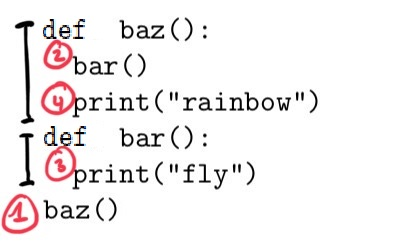
\includegraphics[width=.4\textwidth]{1-trace-calls.jpeg}

In our trace we draw lines next to the functions to have a clear separation, and we number the lines in order of execution. We see that ``fly'' is printed before ``rainbow''.
